\section{Technical}\label{sec:technical}

\subsection{Inference Rules}
Previous work takes advantage of model-checking approach to check whether a
specific C/C++11 trace is sequentially consistent. By estabishing edges
(\textit{sb}, \textit{rf} and \textit{sc} by implication rules) between atomic
operations, it judges whether the trace is SC by whether there exists a cycle in
that graph. 

Under the C/C++11 memory model, inferring the ordering parameters to obtain SC
behaviors is essentially a searching problem. In the absence of consume
operations, memory order parameters for atomic operations can be only one of the
following: \textit{memory\_order\_relaxed}, \textit{memory\_order\_release},
\textit{memory\_order\_acquire}, \textit{memory\_order\_acq\_rel} and
\textit{memory\_order\_seq\_cst}. By enumerating all possible memory order
parameters, we can guarantee that we can find out all the possible inference of
parameters that ensure SC behaviors for a specific test case. However, this
naive approach obviously leads to an exponential searching space.

Consider we start from the case where all memory order parameters are
\textit{memory\_order\_relaxed}. Whenever the model-checking approach finds out
a cycle in a specific execution, we have to infer some stronger memory orders to
eliminate the cycle. In order to guarantee completeness, we propose a
search-based approach combined with patterns to reduce searching space.  In
Figure~\ref{fig:fence_implications} , we show a number of common patterns that
can exist in cycles. We explain what the weakest orders we should impose on
operations to eliminate the corresponding cycle as the following.

\mypara{\bf Synchronization:} This pattern considers 

\mypara{\bf Circular reads-from:}


\mypara{\bf Peterson lock:}


\mypara{\bf Release sequence:}


\mypara{\bf Independent reads \& independent writes:}


Figure~\ref{fig:algorithm} shows the core searching algorithm for all possible
parameters.

\begin{figure}[!ht]
\centering
\begin{tabular}{c}
\multicolumn{1}{c}{Synchronization}\\
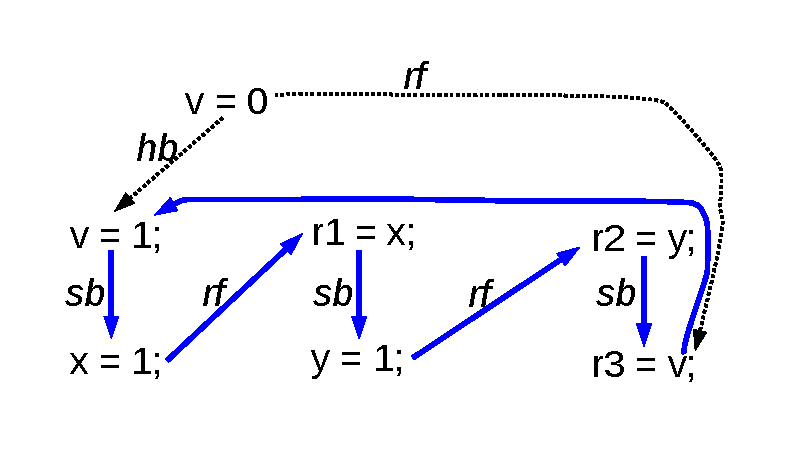
\includegraphics[scale=.4]{figures/sync}\\
\multicolumn{1}{c}{Circular Reads-from}\\
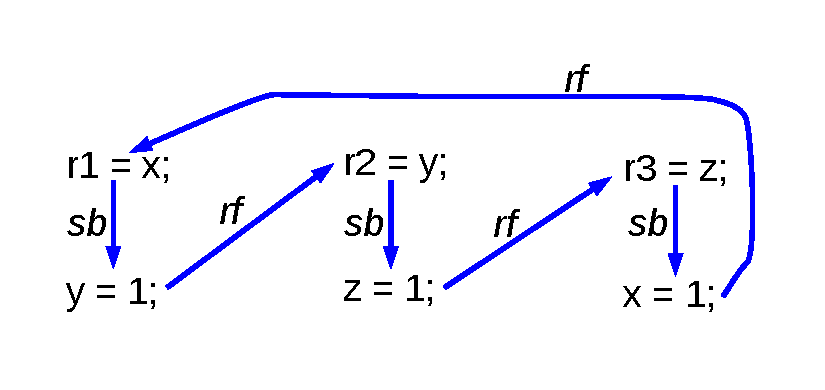
\includegraphics[scale=.4]{figures/circular_rf}\\
\multicolumn{1}{c}{Peterson Lock}\\
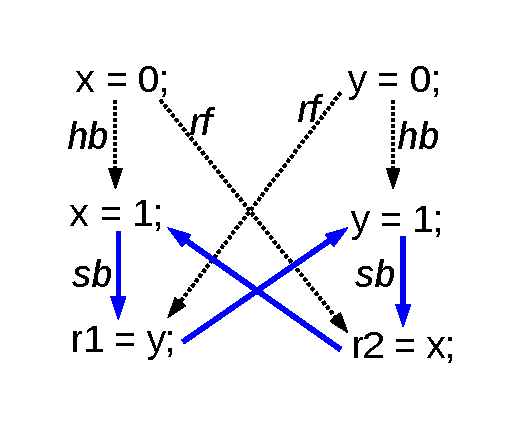
\includegraphics[scale=.4]{figures/peterson_lock}\\
\multicolumn{1}{c}{Release Sequence}\\
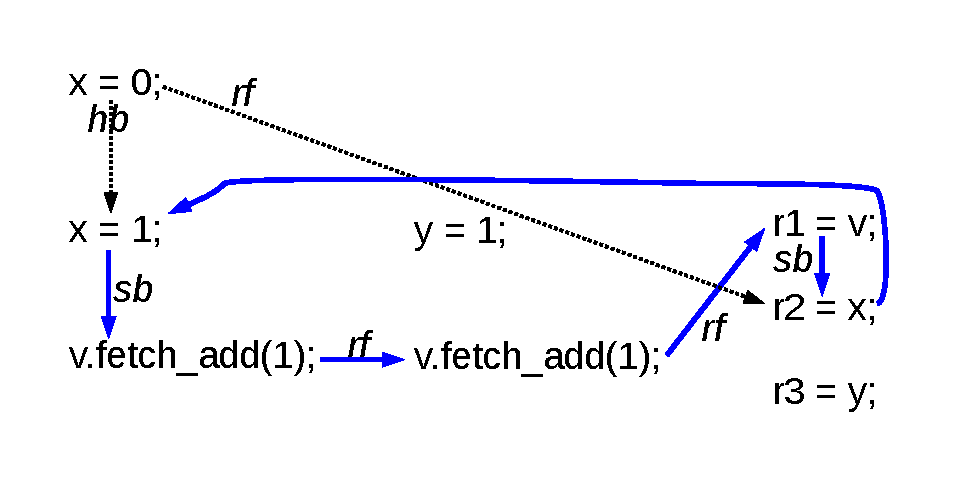
\includegraphics[scale=.4]{figures/release_seq}\\
\multicolumn{1}{c}{Independent Reads \& Independent Writes}\\
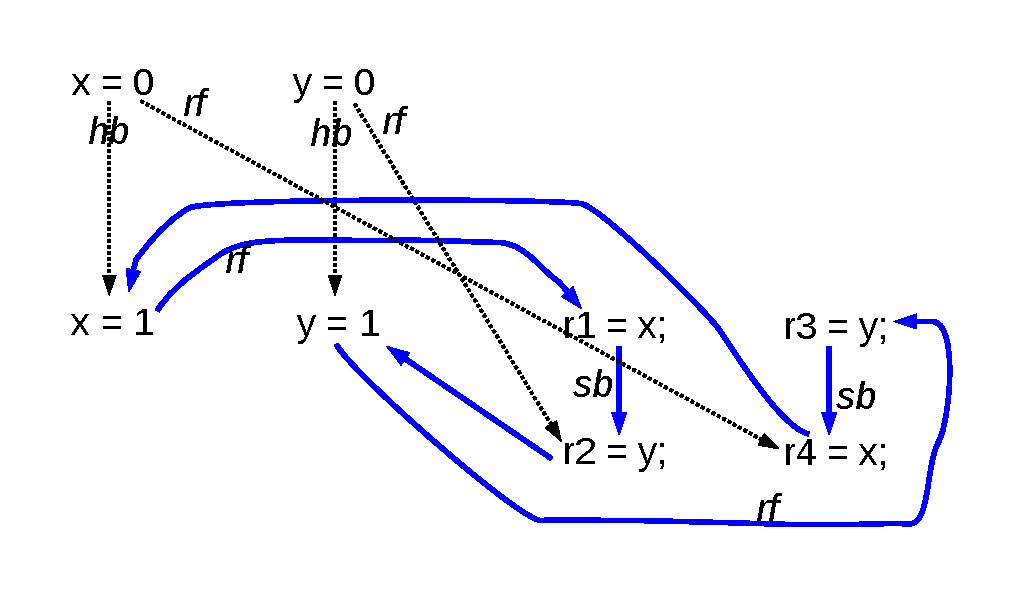
\includegraphics[scale=.4]{figures/iriw}\\
\end{tabular}
\caption{\label{fig:fence_implications}Cycle Patterns for Non-SC Behaviors}
\end{figure}


\begin{figure}[!htbp]
\begin{algorithmic}[1]
\Function{InferParams}{}
\State candidates := \{\}
\State candidate $c1$ := replace all wildcards with \textit{relaxed}
\State candidates += $c1$
\State results := \{\}
\While{candidates is not empty}
\State Candidate $c$ := candidates.pop()
\State Model-check with $c$ and yield a cycle $l$
\If{$l$ == NULL}
\State results += $c$
\Else
\State \Call {StrengthenParam}{$l$, $c$, candidates}
\EndIf
\EndWhile
\State \Return{results}
\EndFunction

\Procedure{StrengthenParam}{cycle, candidate, candidates}
\If{$\exists$ a pattern $p$ in $c$}
\State Candidate new := strengthen $c$ by pattern $p$
\State candidates += new 
\Else
\ForAll{wildcard $w$ in $c$}
\If{$w$ can be strengthened}
\State Candidate new := strengthen $w$ in $c$
\State candidates += new
\EndIf
\EndFor
\EndIf
\EndProcedure

\end{algorithmic}
\caption{\label{fig:algorithm}Algorithm for Searching All Possible Parameters}
\end{figure}

